\documentclass[PhD-Yoann-Dupont.tex]{subfiles}
\begin{document}

%Il est bien connu que pour maximiser la f-mesure, il faut se concentrer sur les entités les plus fréquentes car elles ont plus de poids sur le score global que les entités peu fréquentes.
Le SER, ainsi que la f-mesure, sont des mesures qui favorisent les entités les plus fréquentes, ces dernières ayant plus de poids sur la métrique globale par effet de volume. Détailler les scores entité par entité permet de voir sur quelles entités un système se comporte mieux ou moins bien, mais ne permet pas d'avoir une idée précise quant aux endroits où des gains peuvent être obtenus. Afin de combler ce manque, nous avons calculé, pour chaque entité, son \emph{manque à gagner}. Ce manque à gagner est, pour chaque entité, le nombre de points qui seraient ajoutés à la f-mesure globale si nous la reconnaissions parfaitement. Cela permet d'avoir une meilleure idée des défauts de nos systèmes, cette mesure montrant où et en quelle quantité des gains sont possibles.
Le tableau \ref{tab:fscore-shortfalls} donnent les entités sur lesquelles le manque à gagner en termes de f-mesure est le plus grand.

%We see in the tables that shortfalls gather on leaves or on major types (\emph{amount}, \emph{org}, \emph{pers}). If we perfectly annotated the entities of these tables, we would obtain about 90 in absolute F1-score. We can see that gains are hard to make by focusing on a single entity: if we wanted to gain a single F1-score point that way, this would equate to gaining 10 points on \emph{name} components, 20 on \emph{org.ind} or 24 or \emph{kind}. However, just as errors propagate, corrections would also propagate: \emph{name} being a component of multiple entities, corrections on that component would also spread on the entities above it and would improve scores on multiple entities (for example \emph{org}, \emph{loc} and \emph{pers} where most ambiguities happen at the component level).
Nous remarquons que les manques à gagner se concentrent principalement autour des feuilles ou des entités majoritaires (amount, org, pers). À supposer que toutes les entités du tableau \ref{tab:fscore-shortfalls} soient parfaitement annotées, nous serions à plus de 90 de f-mesure. Nous voyons que les gains ne sont pas aisés à acquérir si l'on se concentre sur un seul type : supposons que nous souhaitions gagner 1 point de f-mesure globale. Cela équivaudrait à un gain d'environ 10 points sur le composant ``name'', 20 sur l'entité ``org.ind'' ou 24 sur le composant ``kind''. Cependant, autant les erreurs se propagent, autant les corrections feraient de même. \emph{name} est un composant de plusieurs entités et ambigu avec les autres composants \emph{name.first} et \emph{name.last}. Des corrections sur ces composants se propageraient sur les entités de niveaux supérieurs, améliorant ainsi la qualité de plusieurs entités en même temps (par exemple \emph{org}, \emph{loc} and \emph{pers} où la plupart des ambiguïtés ont lieu).

\begin{table}[ht!]
    \centering
    \begin{tabular}{|l|c|c|}
    \hline
    entité    & F-mesure & manque à gagner \\
    \hline
    name      & 81.48 & 2.28 \\
    org.ind   & 65.12 & 2.25 \\
    amount    & 75.48 & 2.17 \\
    kind      & 51.20 & 1.97 \\
    qualifier & 49.51 & 1.73 \\
    object    & 76.03 & 1.7  \\
    pers.coll & 59.91 & 1.68 \\
    pers.ind  & 78.05 & 1.4  \\
    \hline
    \end{tabular}
\caption{les entités ayant les plus grands manques à gagner.}
\label{tab:fscore-shortfalls}
\end{table}

Afin de faciliter l'analyse des erreurs, nous avons tiré parti de la classification rafinée des erreurs du SER de la campagne Quaero. Nous avons donc utilisé cinq types d'erreurs : les erreurs de type, de frontière, de type et frontière en même temps, et le bruit. Les entités de référence qui n'ont pu être alignées avec une proposition du CRF sont classées comme étant du silence. Ces scores sont donnés dans le tableau \ref{tab:error-types}. %Cette classification est plus fine que le SER, qui ne considère que les trois types d'erreurs suivants : substitutions (type, frontière, type+frontière), les insertions (bruit) et les suppressions (silence).

\begin{table}[ht!]
\centering
\begin{tabular}{|l|c|}
\hline
type d'erreur      & proportion (\%) \\
\hline
type & 8.0 \\
frontière & 11.7 \\
type+frontière    & 6.2 \\
bruit & 21.6 \\
silence & 52.5 \\
\hline
\end{tabular}
\caption{Pourcentages bruts des différents types d'erreurs.}
\label{tab:error-types}
\end{table}

Le problème principal de notre système est son silence, qui équivaut à 50\% des erreurs du système, 19\% des annotations n'ont aucune proposition faite par le CRF. Le second problème rencontré est la déduction des frontières des entités inconnues, qui représentent presque la moitié des erreurs de précision sur ces dernières. Avec notre classification, il est possible d'explorer plus avant les erreurs faites par notre système, afin de mieux connaître les plus fréquentes et d'avoir des pistes pour les corriger.

%Now, we detail the most common errors made by our system. First, examples of such errors are given in the Table\ \ref{tab:component-errors-examples} for \emph{components}. Errors on entities being mainly propagated, we will focus on component errors. %, and of table \ref{tab:entity-errors-examples} for \emph{entities}.
Nous détaillons maintenant les erreurs les plus communes faites par notre système. Des exemples d'erreurs de frontière, type, bruit et silence donnés respectivement dans les tableaux \ref{tab:component-boundary-examples}, \ref{tab:component-type-examples}, \ref{tab:component-noise-examples} et  \ref{tab:component-silence-examples} pour les composants. Les erreurs sur les entités étant principalement propoagées, nous nous concentrerons sur l'analyse des erreurs sur les composants.

\begin{table}[ht!]
\centering
\small
\begin{tabular}{|p{0.26\linewidth}|p{0.22\linewidth}|p{0.42\linewidth}|}
\hline
description                                                 & CRF & référence \\
\hline
dérivés peu fréquents & $\bullet$ affaires étrangères & $\bullet$ affaires étrangères et de la coopération \\
d'entités fréquentes  & $\bullet$ Afrique             & $\bullet$ Afrique de l'Ouest \\
\hline
composant \textit{object} : ajout ou oubli d'adjectif ou de groupe prépositionnel & emprisonnement & emprisonnement avec sursis \\
\hline
\end{tabular}
\caption{Exemples d'erreurs de frontière.}
\label{tab:component-boundary-examples}
\end{table}

\begin{table}[ht!]
\centering
\begin{tabular}{|p{0.3\linewidth}|p{0.3\linewidth}|p{0.3\linewidth}|}
\hline
description                                                 & CRF & référence \\
\hline
kind vs func                                                                             & \multicolumn{2}{c|}{«~armée~», «~forces~», «~troupes~», «~autorités~», annotés} \\
                                                                                         & \multicolumn{2}{c|}{kind ou func dans les mêmes contextes} \\
\hline
name $\rightarrow$ kind : les composants name deviennent kind avec d'autres composants   & au sein du gouvernement$_{\textcolor{red}{name}}$ israélien$_{demonym}$ & au sein du gouvernement$_{\textcolor{blue}{kind}}$ israélien$_{demonym}$ \\
\hline
\end{tabular}
\caption{Exemples d'erreurs de type sur le Quaero.}
\label{tab:component-type-examples}
\end{table}

\begin{table}[ht!]
\centering
\begin{tabular}{|p{0.3\linewidth}|p{0.3\linewidth}|p{0.3\linewidth}|}
\hline
description                                                 & CRF & référence \\
\hline
composant val: erreur d'analyse sur ``des'', ``de'' et ``d' '' (+erreurs humaines ?) & tirs \textcolor{red}{de} roquettes & tirs de roquettes \\
\hline
composant object : tokens génériques & 2 sets$_{\textcolor{red}{object}}$ à 1 & 2 sets$_{\textcolor{blue}{O}}$ à 1 \\
\hline
composants name : composants vus dans le corpus d'apprentissage & \multicolumn{2}{c|}{pays, valeurs (nombres en chiffres), temps relatif}\\
\hline
\end{tabular}
\caption{Exemples d'erreurs de bruit sur le Quaero.}
\label{tab:component-noise-examples}
\end{table}

\begin{table}[ht!]
\centering
\begin{tabular}{|p{0.4\linewidth}|p{0.25\linewidth}|p{0.25\linewidth}|}
\hline
description                                                        & CRF & référence \\
\hline
composant \textit{val} : oublié sur des montants génériques        & des$_{\textcolor{red}{O}}$ actes de sabotage & des$_{\textcolor{blue}{val}}$ actes de sabotage\\
\hline
composant \textit{qualifier} : oublié si composant qualifié oublié & présumés$_{\textcolor{red}{O}}$ sympathisants & présumés$_{\textcolor{blue}{qualifier}}$ sympathisants \\
\hline
composant \textit{name} : oublié sur temps relatifs                & lendemain$_{\textcolor{red}{O}}$ & lendemain$_{\textcolor{blue}{name}}$ \\
\hline
composant \textit{kind} : noms communs polysémiques                & état$_{\textcolor{red}{O}}$ & état$_{\textcolor{blue}{kind}}$ \\
\hline
\end{tabular}
\caption{Exemples d'erreurs de silence sur le Quaero.}
\label{tab:component-silence-examples}
\end{table}

\begin{comment}
\begin{figure}[ht!]
\centering
\begin{table}{c|p{0.7\linewidth}}
\hline
\multicolumn{1}{c|}{type}    & \multicolumn{1}{|c}{description} \\
\hline
\multirow{2}{*}{boundary} & – \emph{amount} : propagated error \\
 & – \emph{pers.ind} : propagated silence error on component \\
 & – \emph{time.date.rel} : component silence error propagation \\
\hline
\multirow{1}{*}{type} & – \emph{loc.town} vs \emph{pers.ind} : \emph{name} vs \emph{name.first} or \emph{name.last} \\
\hline
\multirow{2}{*}{noise} & – propagated error \\
 & – entities that are both location and organisation (+human errors ?) \\
\hline
\multirow{4}{*}{silence} & – \emph{pers.coll} using common nouns \\
 & – \emph{pers.coll} using singular noun \\
 & – \emph{amount} on generic groups of people or objects \\
 & – \emph{org.ind} : locations not recognised as organisations \\
\hline
\end{table}
\caption{Error overview on entities.}
\label{tab:entity-errors-examples}
\end{figure}
\end{comment}

Comme illustré sur la figure \ref{fig:type-errors-components}, la majorité des erreurs de bruits concernent les composants \emph{func}, \emph{kind} or \emph{name}. Lors de la transition de Quaero v1 à v2, certains composant \emph{kind} ont été remplacés par des composants \emph{func} (cf. Figure \ref{fig:Quaerov1-vs-v2}) : ce sont des composants proches sémantiquement, nous avons également trouvé de potentielles erreurs humaines qui expliqueraient en partie la confusion entre les deux. Quelques erreurs viennent du fait qu'un composant \emph{name} peut devenir \emph{kind} en présence d'autres composants (par exemple, le gouvernement d'un pays). Les CRF semblent avoir du mal à modéliser la présence ou l'absence de ce type de contexte. Toujours en prenant l'exemple des gouvernements, il existe des disparités entre les annotations de référence et les sorties du CRF : bien que ces derniers soient annotés \emph{name} la plupart du temps, cette annotation ne représente que 20\% des sorties du CRF. Des règles de post-traitement pourraient aider à corriger ce type d'erreurs.
%On the chart of Figure \ref{fig:type-errors-entities}, it can be seen that errors on types involve mostly \emph{org}, \emph{pers} and \emph{loc}. Those errors involving \emph{pers} are propagated errors: they all have a \emph{name} component, but different types. A person always has a subclass of \emph{name}, while \emph{loc} and \emph{org} do not, meaning that if a first name was badly identified, the system will then identify a location or an organisation instead of a person. Our system also seems to have a problem identifying Arab names in general.

Le plupart des erreurs de silence sont faites sur les composants de Quaero, représentant 60\% de l'ensemble des erreurs de silence faites par le CRF. Ces dernières sont faites principalement sur les composants \emph{val}, \emph{object}, \emph{kind} et \emph{qualifier}. \emph{Object} étant un composant de l'entité \emph{amount}, il est lié au composant \emph{val}, ce qui explique en partie le phénomène, même si nous n'avons pas pu le quantifier de manière précise. Les erreurs faites sur les composants \emph{qualifier} sont uniquement contextuelles, ce composant n'apparaissant jamais seul, la plupart des silences étant dûs au silence sur l'élément qualifié. Il semble donc que le CRF ait été capable de modéliser cette contrainte, signifiant que ces silences peuvent être corrigés si nous parvenons à identifier l'élément qualifié.

%Boundary errors on components are usually of length 1 or 2 and seem equally distributed between additions and deletions, they mostly are adjectives or prepositional phrases. When it comes to entities, boundary errors tend to be larger on overall, this is due to the propagation of two kinds of errors: first the boundary errors on some components will cause an entity to have a boundary error also. Second, a silence error on a component can lead to a boundary error in an entity, for example when a first/last name is not identified at a component level, but the person is still identified.
Les erreurs de frontière sur les composants sont généralement de taille 1 à 2 et sont plus ou moins équitablement distribuées entre les ajouts et les suppressions. Ces erreurs de frontières concernent principalement des adjectifs et des groupes prépositionnels. Pour les entités, les erreurs de frontière tendent à devenir plus grandes, cela est dû à la propagation de deux types d'erreurs. Premièrement, les erreurs de frontières sur les composants vont causer une erreur de frontière sur l'entité au-dessus d'eux. Deuxièmement, une erreur de silence peut conduire à une erreur de frontière sur une entité. Par exemple, si seul un nom de famille ou un prénom est reconnu pour une personne, la personne pourra malgré tout être identifiée, mais une de ses frontières sera incorrecte.

%Most noise errors are on components such as \emph{val}, \emph{object}, \emph{kind}, \emph{qualifier} and \emph{name}. Nearly 80\% of those noise errors are on components whose form was observed on the training corpus. While some are most likely human errors, such as countries and proper names, some others are more contextual and may indicate an overfitting of the CRF, that just took those components ``at face value''.
La plupart des erreurs de bruit sont sur les composants \emph{val}, \emph{object}, \emph{kind}, \emph{qualifier} et \emph{name}. Presque 80\% de ces erreurs de bruit sont sur des composants dont la forme a été observée dans le corpus d'entrainement. Même si certaines sont très probablement des erreurs humaines (sur des pays et des noms propres principalement), certaines sont plus spécifiques et semblent indiquer un surapprentissage du CRF, qui utilise la forme pour identifier certains composants.

\begin{figure}
\begin{minipage}{0.49\linewidth}
    \centering
    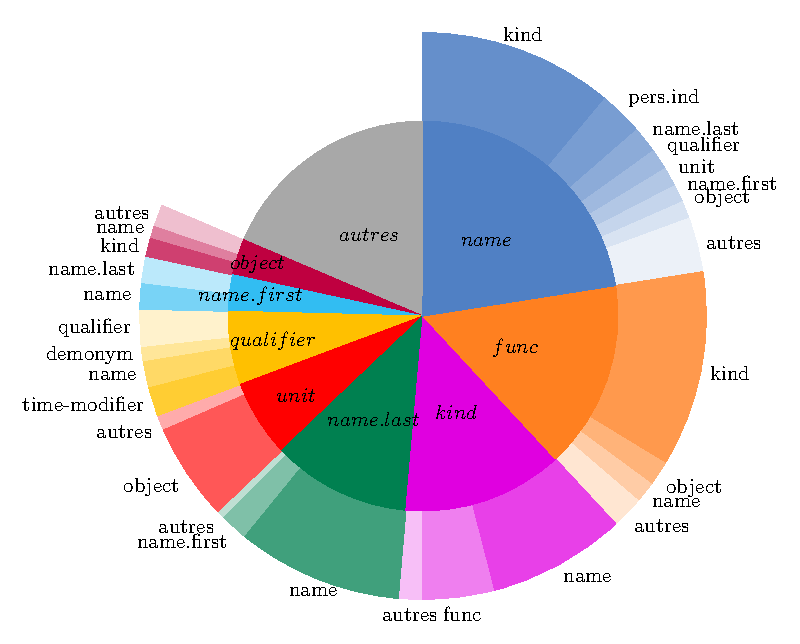
\includegraphics[scale=0.6]{images/quaero/components-type}
\end{minipage}
\begin{minipage}{0.49\linewidth}
    \centering
    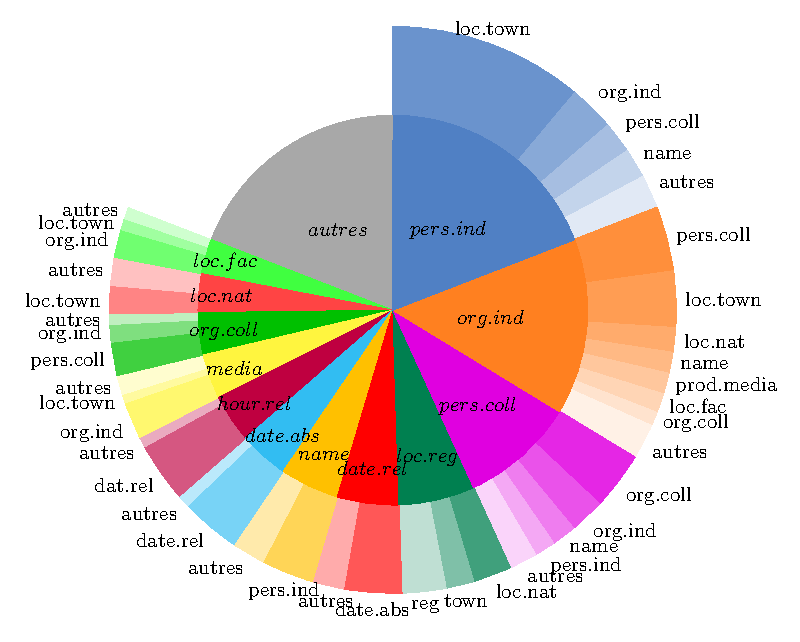
\includegraphics[scale=0.6]{images/quaero/entities-type}
\end{minipage}
\caption{Erreurs de type. À gauche sur les composants, à droite sur les entités. La partie intérieure correspond au type de la référence. La partie supérieure correspond au type donné par le système.}
\label{fig:type-errors-components}
\end{figure}

%As previously showed, most errors on entities seem to originate from errors made on previous levels. To check this assertion, we tried a run using the reference components instead of using a CRF to annotate leaf level components in algorithm \ref{alg:CRFcascade}: the SER dropped to 6.3\%, a result coherent with the one stated by \cite{Dinarelli2011}, who made the same test (Table 4). We plan to isolate non-propagated type-specific errors to analyse them specifically in further research. This last test provides a strong proof that we should focus more on components of the first level, especially for common nouns that tend to be more ambiguous than proper nouns. We also need to model some ``horizontal'' structuration better: some components work ``symbiotically'' with others, such as \emph{val} and \emph{object}. Type errors also showed the need for a better disambiguation between the different \emph{name} components.
Comme nous l'avons montré précédemment, la plupart des erreurs sur les entités semblent venir d'erreurs faites à des niveaux inférieurs. Pour valider cette assertion, nous avons lancé une annotation en reprenant les annotations de référence pour les composants du premier niveau au lieu d'effectuer une annotation avec un CRF comme indiqué dans l'algorithme \ref{alg:AnnotationCascade} : le SER est passé à 6.3\%. Ce résultat est cohérent avec celui de \cite{Dinarelli2011}, qui avait effectué le même test (tableau 4 dans l'article). Nous prévoyons d'isoler les erreurs non propagées pour chaque type afin de mieux comprendre l'influence de la propagation des erreurs ainsi que des erreurs dûs à des manques intrinsèques au CRF dans son état actuel. Nous avons également besoin de mieux modéliser le contexte afin mieux désambiguiser les composants \emph{name}.

\end{document}